\documentclass{article}

\usepackage{graphicx} % Required for inserting images
\usepackage[left=1in,right=1in,top=1in,bottom=1in]{geometry}
\usepackage{amsmath}
\usepackage{amsthm} %proof environment
\usepackage{amssymb}
\usepackage{amsfonts}
\usepackage{enumitem} %nice lists
\usepackage{verbatim} %useful for something 
\usepackage{xcolor} \usepackage{setspace}
\usepackage{titlesec}
\usepackage{blindtext} % I have no idea what this is 
\usepackage{caption}  % need this for unnumbered captions/figures
\usepackage{natbib}
\usepackage{tikz}
\usepackage{hyperref}

\titleformat{\section}{\bfseries\Large}{Problem \thesection:}{5pt}{}

\begin{document}

\title{AM 275 - Magnetohydrodynamics:}
\author{Dante Buhl}


\newcommand{\wrms}{w_{\text{rms}}}
\newcommand{\bs}[1]{\boldsymbol{#1}}
\newcommand{\tb}[1]{\textbf{#1}}
\newcommand{\bmp}[1]{\begin{minipage}{#1\textwidth}}
\newcommand{\emp}{\end{minipage}}
\newcommand{\R}{\mathbb{R}}
\newcommand{\C}{\mathbb{C}}
\newcommand{\N}{\mathcal{N}}
\newcommand{\K}{\bs{\mathrm{K}}}
\newcommand{\m}{\bs{\mu}_*}
\newcommand{\s}{\bs{\Sigma}_*}
\newcommand{\dt}{\Delta t}
\newcommand{\dx}{\Delta x}
\newcommand{\tr}[1]{\text{Tr}(#1)}
\newcommand{\Tr}[1]{\text{Tr}(#1)}
\newcommand{\Div}{\nabla \cdot}
\renewcommand{\div}{\nabla \cdot}
\newcommand{\Curl}{\nabla \times}
\newcommand{\Grad}{\nabla}
\newcommand{\grad}{\nabla}
\newcommand{\grads}{\nabla_s}
\newcommand{\gradf}{\nabla_f}
\newcommand{\xs}{x_s}
\newcommand{\xf}{x_f}
\newcommand{\ts}{t_s}
\newcommand{\tf}{t_f}
\newcommand{\pt}{\partial t}
\newcommand{\pz}{\partial z}
\newcommand{\uvec}{\bs{u}}
\newcommand{\bvec}{\bs{B}}
\newcommand{\B}{\bs{B}}
\newcommand{\jvec}{\bs{j}}
\newcommand{\F}{\bs{F}}
\newcommand{\T}{\tilde{T}}
\newcommand{\ez}{\bs{e}_z}
\newcommand{\ex}{\bs{e}_x}
\newcommand{\ey}{\bs{e}_y}
\newcommand{\eo}{\bs{e}_{\bs{\Omega}}}
\newcommand{\ppt}[1]{\frac{\partial #1}{\partial t}}
\newcommand{\pp}[2]{\frac{\partial #1}{\partial #2}}
\newcommand{\pptwo}[2]{\frac{\partial^2 #1}{\partial #2^2}}
\newcommand{\DDt}[1]{\frac{D #1}{D t}}
\newcommand{\ppts}[1]{\frac{\partial #1}{\partial t_s}}
\newcommand{\pptf}[1]{\frac{\partial #1}{\partial t_f}}
\newcommand{\ppz}[1]{\frac{\partial #1}{\partial z}}
\newcommand{\ddz}[1]{\frac{d #1}{d z}}
\newcommand{\ppzetas}[1]{\frac{\partial^2 #1}{\partial \zeta^2}}
\newcommand{\ppzs}[1]{\frac{\partial #1}{\partial z_s}}
\newcommand{\ppzf}[1]{\frac{\partial #1}{\partial z_f}}
\newcommand{\ppx}[1]{\frac{\partial #1}{\partial x}}
\newcommand{\ppxi}[1]{\frac{\partial #1}{\partial x_i}}
\newcommand{\ppxj}[1]{\frac{\partial #1}{\partial x_j}}
\newcommand{\ppy}[1]{\frac{\partial #1}{\partial y}}
\newcommand{\ppzeta}[1]{\frac{\partial #1}{\partial \zeta}}


\maketitle 
% This line removes the automatic indentation on new paragraphs
\setlength{\parindent}{0pt}

\section{Magnetic Field Lines}

Here is a figure \ref{fig:p1} of the magnetic field lines, and following is a plot of the
field lines. 

\begin{figure}
    \centering
    \includegraphics[width=.8\textwidth]{field_line.jpg}
    \caption{Drawing of magnetic field lines}
    \label{fig:p1}
\end{figure}


\section{Oscillating Magnetic Field Diffusion}

Solve the given PDE for a magnetic field in a semi-infinite volume ($z > 0$)
with high resistivity ($\eta$), and the following boundary condition,
\begin{gather*}
    \B(z=0,t) = \left(B_0e^{-i\omega t}, 0, 0\right)
\end{gather*}

\begin{proof}
    We begin by demonstrating that since this is a linear problem, we have that
    the conditions at $z = 0$, and $t = 0$ (taken by setting $t = 0$ in the BC),
    that the $y$ and $z$-components of the magnetic field will be constant ($ =
    0$) for all $t \ge 0$. 
    \begin{gather*}
        \ppt{B_y}(t = 0) = \eta \grad^2B_y(t = 0) = 0\\
        \ppt{B_z}(t = 0) = \eta \grad^2B_z(t = 0) = 0
    \end{gather*}
    and so they must remain zero for all time. Thus we have shown that the
    problem is reduced to the following equation, 
    \begin{gather*}
        \ppt{B_x} = \eta \grad^2B_x, \quad B_x(z,t)\\
        \ppt{B_x} = \eta \pptwo{B_x}{z}, \quad B_x(z=0,t) = B_0e^{-i\omega t},
        \quad B_x(z\to\infty,t) = 0, \quad B_x(z, t=0) = B_0
    \end{gather*}
    We begin by solving using a separation of variables solution in $z$ and
    $t$. 
    \begin{gather*}
        B_x = Z(z)T(t), \quad \frac{T'}{\eta T} = \frac{Z''}{Z} = -c^2
    \end{gather*}
    here in order to satisfy the boundary conditions, we will take $c$ to be
    complex valued, i.e. $c = \alpha + i\beta$. We begin solving these ODEs starting with
    $Z$. 
    \begin{gather*}
        Z'' = -c^2Z \implies Z(z) = c_1e^{icz} + c_2e^{-icz}\\
        Z(z) = e^{-\beta z}\left(a_1\cos(\alpha z) + b_1\sin(\alpha z)\right) +
        e^{\beta z}\left(a_2\cos(\alpha z) + b_2\sin(\alpha z)\right) \\
        Z(0) = 1 \implies a_1 + a_2 = 1\\
        \lim_{z\to\infty}Z(z) = 0 \implies a_2 = b_2 = 0\\
        Z(z) = e^{-\beta z}\left(\cos(\alpha z) + b_1\sin(\alpha z)\right)
    \end{gather*}
    Next we move to the ODE for time. We have, 
    \begin{gather*}
        T' = -c^2\eta T \implies T = T_0e^{-c^2\eta t}, \quad -c^2 = \beta^2 -
        \alpha^2 -  i2\alpha\beta \\
        T = T_0e^{-(\beta^2 - \alpha^2)\eta t}\left(\cos(2\alpha\beta\eta t)
        - i\sin(2\alpha\beta\eta t)\right)\\
        T(t=0) = T_0 = B_0
    \end{gather*}
    Next we put these two separable solutions together and solve for the last
    BC,
    \begin{gather*}
        u(z=0,t) = B_0e^{-(\beta^2-\alpha^2)\eta t}\left(\cos(2\alpha\beta\eta t)
        - i\sin(2\alpha\beta\eta t)\right) = B_0e^{-i\omega t} \\
        \implies \beta^2 - \alpha^2 = 0, \quad \alpha = \pm \beta \\
        2\alpha\beta\eta t = \pm 2\alpha^2\eta t = \omega t\\
        \alpha = \sqrt{\frac{\omega}{2\eta}}
    \end{gather*}
    With the eigenvalue solved, we can then write the solution for $B_x$. 
    \begin{gather*}
        B_x = B_0\exp\left(-\sqrt{\frac{\omega}{2\eta}}z - i\omega
        t\right)\left(\cos\left(\sqrt{\frac{\omega}{2\eta}}z\right) + 
        \sin\left(\sqrt{\frac{\omega}{2\eta}}z\right)\right)
    \end{gather*}
    Notice that this solution oscillates on a wavelength of $\lambda = 2\pi/k_z =
    2\pi/\sqrt{\omega/2\eta} = 2\pi\sqrt{2\eta/\omega}$, and the exponential
    decay occurs on a scale height of $L_z = \sqrt{2\eta/\omega}$. 
\end{proof}

\begin{figure}
    \centering
    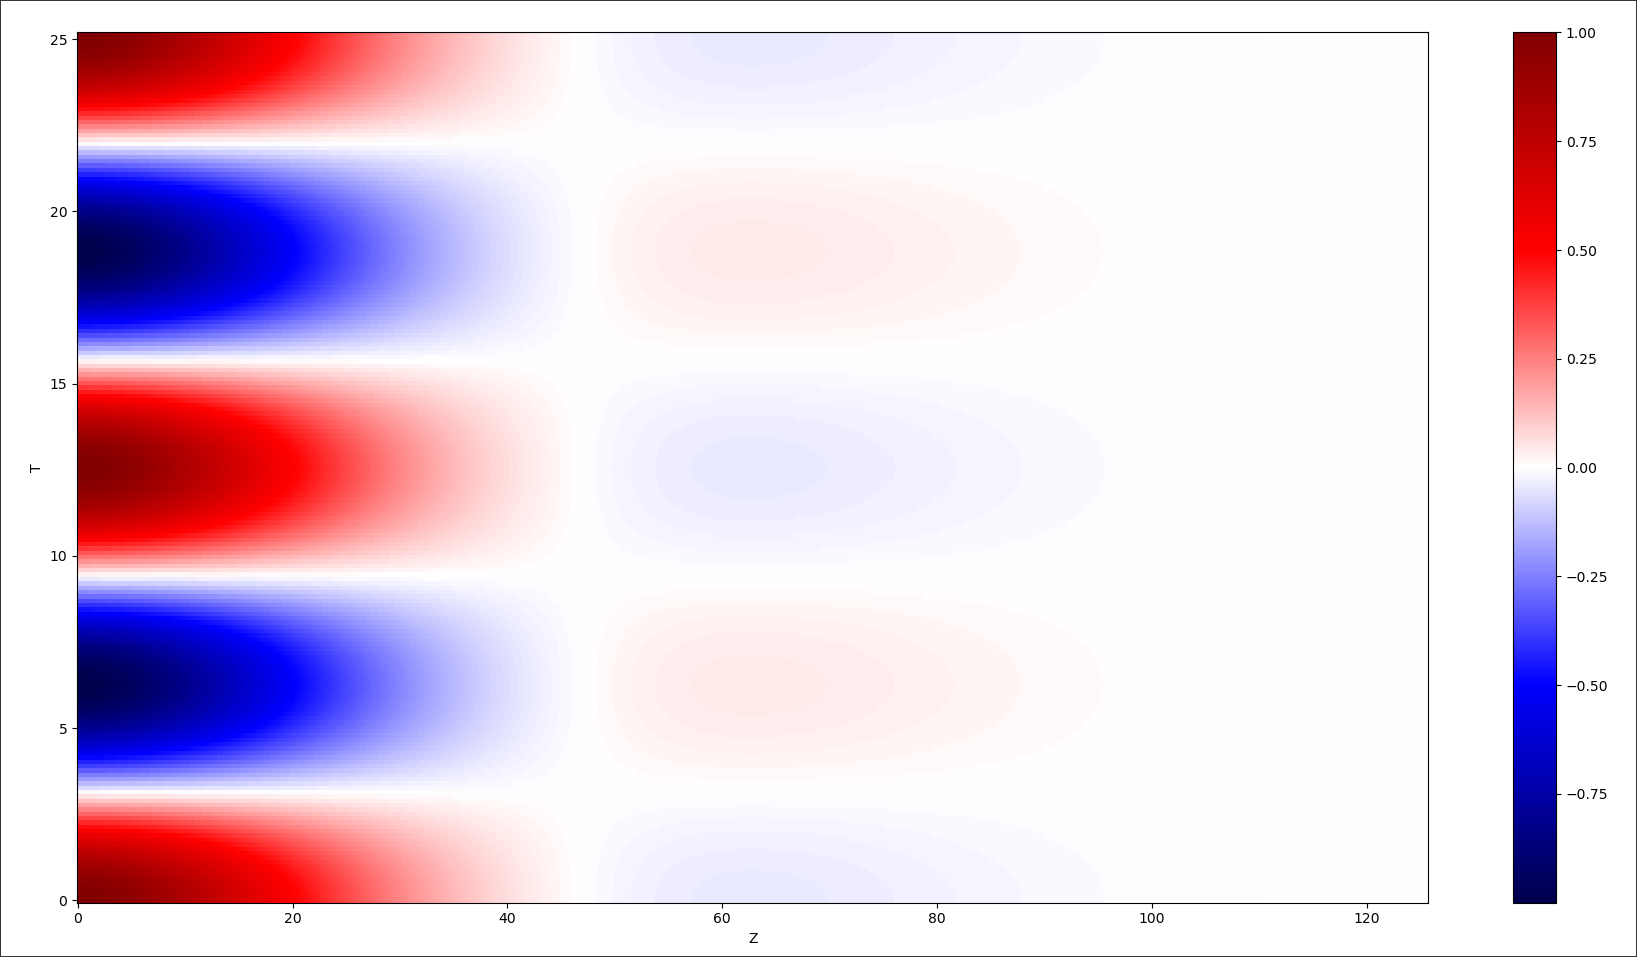
\includegraphics[width=1\textwidth]{hw1p5_plot.png}
    \caption{Plot of solution for problem 2 obtained using python using $\eta =
    100$, $\omega = 0.5$, and $B_0 = 1$.}
\end{figure}





\end{document}
